\documentclass[11pt]{article}
\usepackage[utf8]{inputenc}	% Para caracteres en español
\usepackage{amsmath,amsthm,amsfonts,amssymb,amscd}
\usepackage{multirow,booktabs}
\usepackage[table]{xcolor}
\usepackage{fullpage}
\usepackage{lastpage}
\usepackage{enumitem}
\usepackage{fancyhdr}
\usepackage{mathrsfs}
\usepackage{wrapfig}
\usepackage{setspace}
\usepackage{hyperref}
\usepackage{calc}
\usepackage{multicol}
\usepackage{cancel}
\usepackage[retainorgcmds]{IEEEtrantools}
\usepackage[margin=3cm]{geometry}
\usepackage{amsmath}
\newlength{\tabcont}
\setlength{\parindent}{0.0in}
\setlength{\parskip}{0.05in}
\usepackage{empheq}
\usepackage{framed}
\usepackage[most]{tcolorbox}
\usepackage{xcolor}
\colorlet{shadecolor}{orange!15}
\parindent 0in
\parskip 12pt
\geometry{margin=1in, headsep=0.25in}
\theoremstyle{definition}
\usepackage{pdfpages}
\newtheorem{defn}{Definition}
\newtheorem{reg}{Rule}
\newtheorem{exer}{Exercise}
\newtheorem{note}{Note}
\usepackage{fancyhdr}\usepackage{xcolor}\usepackage{amsmath}\usepackage{amssymb}\pagestyle{fancy}\rhead{}
\newtheorem{theorem}{Theorem}[subsection]
\theoremstyle{definition}
\newtheorem{definition}[theorem]{Definiton}
\newtheorem{example}[theorem]{Example}
\newtheorem{corollary}[theorem]{Corollary}
\newtheorem{lemma}[theorem]{Lemma}
\title{Chapter 9 Review Notes}
\begin{document}
\thispagestyle{empty}
{\LARGE \bf MSE 160 Lecture Notes}\\
{\large Hei Shing Cheung}\\
Molecules and Materials, Winter 2024 \hfill MSE 160\\
\begin{center}
\textit{"In this class we are mostly understanding solids''} \\ - Prof. \textsc{Scott Ramsay}
\end{center}
\vspace{10pt}
\section{Mechanical Behavior}
\paragraph{Classes of Materials} In this class, we look at three classes of materials (non-exhaustive):
\begin{itemize}
    \item \textbf{Metal} held together with metallic bonds, typically \textbf{ductile} and \textbf{conductive}.
    \item \textbf{Ceramics}  (often metal oxides [excp: diamond]) held together via covalent \& ionic bonds, typically \textbf{brittle} and \textbf{insulating}.
    \item \textbf{Polymers} Molecules (often hydrocarbons) typically \textbf{ductile} and \textbf{insulating}
\end{itemize}
\paragraph{Engineering Stress} We know that:
\begin{equation}
    \sigma = \frac{F}{A_0}
\end{equation}
\paragraph{Engineering Strein} Also:
\begin{equation}
    \epsilon = \frac{\Delta l}{l_0}
\end{equation}
\paragraph{Young's Moduclus} For elastic deformation, $E$, is given, by Hooke's Law, as follows:
\begin{equation}
    \sigma = E \epsilon
\end{equation}
\paragraph{Tensile Test} We apply force as to the ends of a dogbone-sample, with $l_0$ being the gauge length and $A_0$ being the area of the cross-section at the middle. 
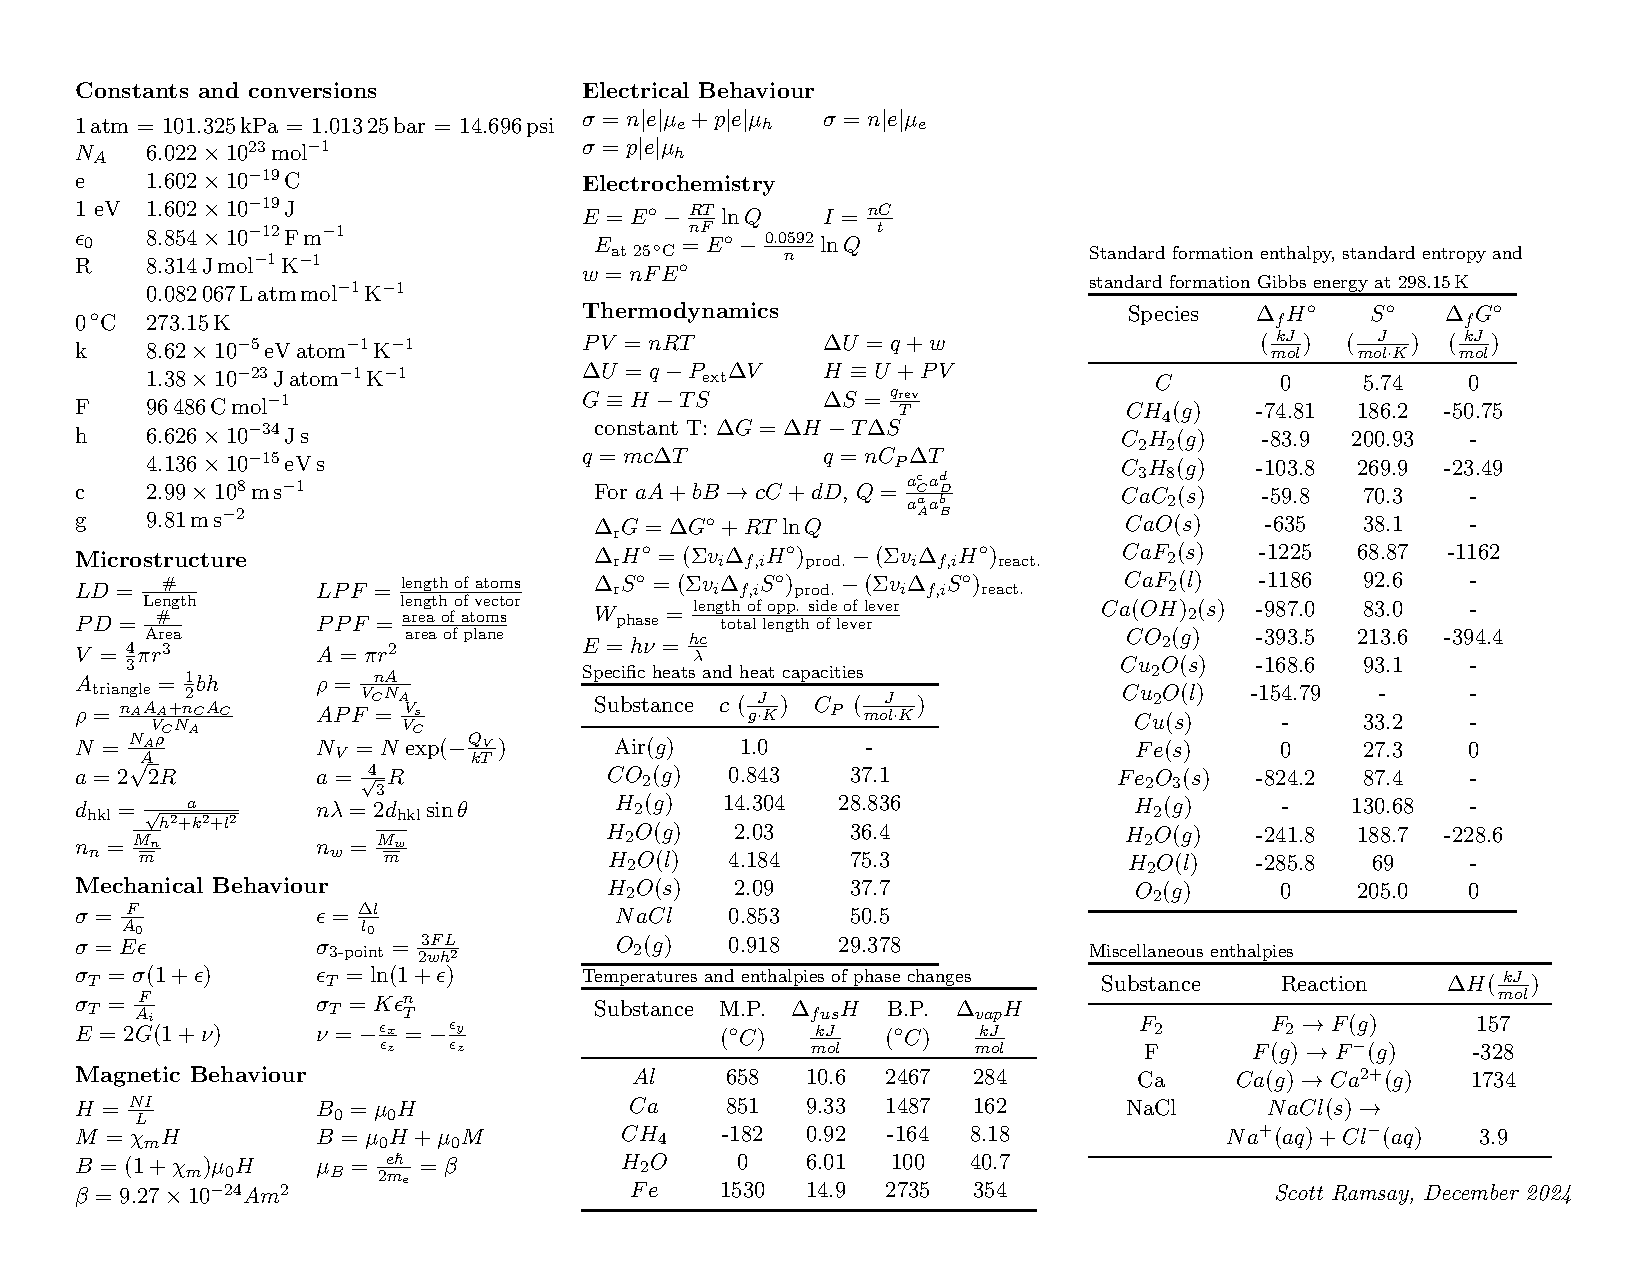
\includepdf[pages=-, angle=90]{EquationSheet.pdf}
\end{document}